\section{Background}\label{chapter.background}
\thispagestyle{plain}
Before moving onto the technical substance, it will be beneficial to acquire a theoretical basis on the subject of this thesis. This chapter introduces software testing and explains some essential concepts. Further, it presents constraint programming and optimization as well as some previous work related to this thesis.

\subsection{Software Testing}

A fundamental understanding of software testing is a useful prerequisite in order to fully understand the context of this thesis. Consequently, this section provides a short introduction to software testing. Since this is a large field, only a small selection of relevant concepts and ideas will be presented. \comment{The testing strategy, process and technique used in this project will also be introduced here.} % and maybe test policy?

Software testing is the process of evaluating the quality of the application, system or component being tested, commonly referred to as the test object or the system under test. Software testing may involve any action oriented toward assessing the software with the goal of determining whether it meets the required results  \cite{[http://istqbexamcertification.com/what-is-a-software-testing/]}.

Software is developed by human beings who can make errors. These errors may cause defects in the source code. Executing defected code can lead to failure in the program  \cite{http://www.istqb.org/downloads/send/2-foundation-level-documents/3-foundation-level-syllabus-2011.html}. One of the purposes of software testing is to examine the test object with the intent of revealing such defects. Other objectives include to measure and ensure quality, and to provide confidence in the product \cite{SoftwareTestingFoundations}.

\subsubsection{The V-Model}\label{sec.v_model}

\begin{figure}[h]
    \centering
    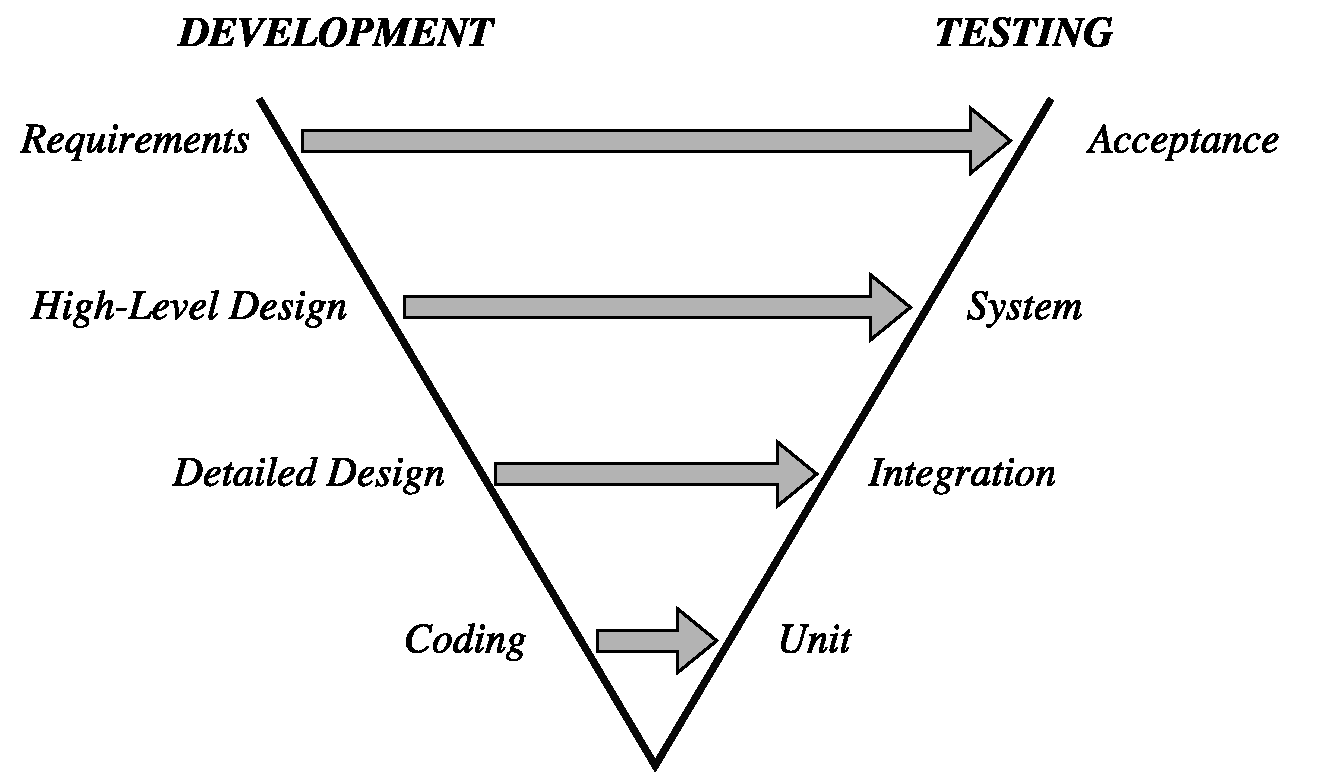
\includegraphics[width=\textwidth]{figures/new/v_model.pdf}
    \caption{The V-Model}
    \label{fig.v-model}
\end{figure}


\noindent The \emph{V-model} is an important asset in software testing, behind which the general idea is to link each development task in a software development process to an equivalent testing task of comparable importance.\comment{ This is symbolized by the two branches of the letter \emph{V} in the model.} The development process is represented by the left branch of the letter \emph{V}, which shows the system being gradually developed. The right branch represents the testing process in which progressively larger subsystems are tested \cite{SoftwareTestingFoundations}.

Depending on the literary source, the V-model covers a varying number of levels. The V-model shown in Figure \ref{fig.v-model} is created using the four levels found in \cite{systematicSoftwareTesting}. The highest development level covers gathering, specification and approval of requirements. Acceptance testing correspondingly checks if these requirements are met. Further, high-level design covers the functional design of the system, and corresponds to system testing, which aims to verify if the system as a whole meets the required results. Detailed design covers technical system design and component specification, and integration testing correspondingly verifies that the different components work together as specified. The lowest level is the coding in which the specified components (modules, units and classes) are implemented. It corresponds to unit and component testing. The tests at this level aim to verify that system components perform as specified, by testing them in isolation  \cite{SoftwareTestingFoundations}.

\comment{
    \begin{Description}
        \setlength{\itemsep}{1pt}
        \setlength{\parskip}{4pt}
        \setlength{\parsep}{0pt}
        \item[\betterfakesc{Requirements} $\Leftrightarrow$ \betterfakesc{Acceptance Test}]\hfill\\
        The requirements are gathered, specified and approved. Acceptance tests check if the requirements as specified in the contract are met. This is the highest development and test level of Figure \ref{fig.v-model}.
        \item[\betterfakesc{High-Level Design} $\Leftrightarrow$ \betterfakesc{System Test}]\hfill\\
        The functional design of the system is covered here. System testing verifies if the system as a whole meets the specified requirements.
        \item[\betterfakesc{Detailed Design} $\Leftrightarrow$ \betterfakesc{Integration Test}]\hfill\\
        Detailed design covers technical system design and component specification. Integration testing correspondingly verifies that the different components work together as specified.
        \item[\betterfakesc{Coding} $\Leftrightarrow$ \betterfakesc{Unit Test}]\hfill\\
        The specified components (modules, units, classes) are implemented. Component testing and unit testing verifies that system components perform as specified by testing them in isolation. This is the lowest development and test level of Figure \ref{fig.v-model}.
    \end{Description}
}

\toolname \space is a tool for high-level test execution, and is intended for the two highest test-levels of the V-model; system testing and acceptance testing.


\subsubsection{Black-Box \& White-Box Testing}
\noindent Software testing can be divided into \emph{black-box} and \emph{white-box} testing. White-box testing is based on analysis of the internal system structure, and requires knowledge of the source code. In black-box testing, the test object is seen as black-box, whose behavior is watched from the outside. The inner structure of the system is either unknown or disregarded. Test cases are determined from the specifications of the system. 

Black-box testing is predominantly used for higher levels of testing. The test object is accessed through the user interface (UI). Tests are performed from the perspective of an end-user, and aim to mimic a human being interacting with the system. Black-box testing includes functional testing, which is used to validate a particular feature for correctness according to the requirements specifications \cite{SoftwareTestingFoundations}.

\toolname \space performs tests by using Selenium, an automation tool that will be introduced in Section \ref{subsec.selenium}, to automate web browsers. It executes functional UI tests on full system builds, and runs without access to or consideration of the source code or the internal system structure. The test method covered by \toolname \space is therefore black-box testing.



\comment{
    [CI - \url{http://stackoverflow.com/questions/17719385/how-to-make-jenkins-run-selenium-webdriver-testng-java-tests-automatically-on-de}]
}

\subsubsection{Test Automation}
As opposed to humans performing software tests manually, test automation is the practice of writing scripts that conduct tests when executed. Automation can be applied to tests at any level. Low-level tests, such as unit and component tests, generally run fast and are durable since they are isolated from changes in other parts of the system. As we move up to the integration level, the tests do not run as fast, and become less durable since they depend on multiple components working together in subsystems. \toolname \space is concerned with testing the system from the perspective of an end-user. Such tests require the system to work as a whole, and thus generally run slower and are more brittle \cite{pluralsight_endtoend} than tests on lower levels.

\comment{PLURALSIGHT lecture: Automated Testing: End To End}

There are a number of strengths to automated tests. They are superior at verifying logical functionality. They can be executed any number of times, and they run more quickly than a human interacting with the system, thus saving time and reducing effort. Time saved on manual testing can be used to increase the test coverage, which can provide reduced risk and higher software quality. Tests and tasks that would be error prone if done manually and tests that are repeatedly performed are typical subjects for automation \cite{ASTvol3}. This includes regression testing, which is used to verify that defects have not been introduced in a new version of previously tested software \cite{SoftwareTestingFoundations}.

Manual human testing has a number of benefits too. Human testers can identify corner cases and check how the system responds when it is used in manners it is not designed to be used for. They can also evaluate aesthetics and design of the UI as well as the overall user experience. Thus, test automation on the two highest levels in the V-model should not be a complete replacement for manual human testing; the two should instead complement each other.

Test automation is often incorporated in \emph{continuous integration} (CI) \cite{ci} environments. This has not been done in this project, but is presented in \ref{further_work.ci} as a suggestion for further work.

\comment{
[What should be automated? What can't be obtained through automated testing?] While automated tests may run quickly and effectively, can be cost-effective and are useful for repeating tests the same way repeatedly, the natural exploration that occurs when humans perform manual testing does not happen through executing automated test scripts. Writing and maintaining test scripts are time-consuming, so it is important to only use resources on automating test cases of value.  Test automation should not replace manual testing as a whole; the two should complement each other through a combination of adequate amounts of both manual and automated testing.
}

\comment{
    "Selenium tests run on a real browser, they need to perform actual browser operations and often wait for an HTTP server to respond. The implication is that if you include Selenium tests as part of your build, the build will take much longer to run - so that if currently you’re running a build on every commit, or several times a day, you may have to resort to running the build overnight, and you might need to upgrade your Jenkins workstation or even add more machines to your Jenkins cluster."
}

\comment{
    IEEE/ISO Standard
    ISTQB Websiden (terminologi etc.)
    Software Testing boken
    
    * Se på test nivåer - må forklare på hvilket nivå disse testene utføres.
    * Se på test tilnæringer - f.ekx. black, white, grey box testing eller context driven testing. Finnes og andre. Sjekk litteratur. Du driver med black/grey box testing hvis man ser det utfra det perspektivet.
    * Se på forskjellige test teknikker/metoder - statisk testing, dynamisk testing, funksjonell vs. icke-funksjonell testing etc.
    * Teststrategi, -policy og -prosess -- input fra Alitbox. Spør hva de har for dokumentasjon rundt dette. Ellers finnes dette i IEEE standard. Fornuftig å skrive at du har valgt en strategi, policy og prosess for tid arbeid. Kanskje strategi og prosess er spesielt viktig. Policy er kanskje ikke nødvendig da det ofte er veldig orgranisasjonsspesifikkt.
    
    
    test strategy-A test strategy is an outline that describes the testing approach of the software development cycle.
    test levels - systemtest, integrasjonstest, akseptansetest osv.
    test metode/teknikk - black, white box testing
    test type - 
    
    non-functional testing - the way the system operates.
    functional testing - what the system does
    
    Functional testing is a quality assurance (QA) process[1] and a type of black-box testing 
}

%%% SUBSECTION: Constraint Programming and Optimization %%%
\subsection{Constraint Programming \& Optimization}\label{subsection.cp}
As explained in the previous section, the type of tests targeted in this project are time-consuming. This means that a large collections of test cases, or test sets, could take unnecessarily long time to execute if the tests were not carefully allocated among the available test machines. Minimizing the execution time of a test run has been an important objective in this project.

There are certain requirements that must be fulfilled upon allocating tests in \toolname. A test that is specified to run in a certain browser can only be allocated to a machine with the given browser installed; this is a constraint. \emph{Constraint programming} (CP) revolves around modelling real-world constraints by mathematical formalizations, and use them to find feasible solutions to the problem \cite{MortensBok}. 

Some problems have very large sets of possible solutions, while others only have a few or none at all. Sometimes it is not enough to simply find a possible solution to a CP problem, as the quality of different solutions can vary greatly. In such cases, a specification of which solutions are more valuable should be provided to help separate the good solutions from those of poor quality. The objective of the CP problem in this project is to minimize the overall execution time of a test run. An \emph{optimization problem} is a CP problem in which such an objective is specified \cite{MortensBok}.

The optimization problem in this project does not exclusively revolve around finding an optimized allocation -- in situations where the problem has a huge number of solutions, identifying the best solution can take a vast amount of time.\comment{For instance, in a situation with two competing solutions where one provided a 10 second longer overall execution time, but took 20 seconds less to find, this would be the preferred solution.} The time taken to find the solution must therefore also be taken into account. Accordingly, some stop criteria for searching must be defined; these will be presented in Chapter \ref{chapter.implementation}.

Formally, the optimization problem in this project considers a set of tests $\cmsy{T} = \{t_{1},\ \dots,\ t_{n}\}$ with a corresponding set of durations $\cmsy{D} = \{d_{1},\ \dots,\ d_{n}\}$ in which the values are derived from the durations of earlier executions of each test. Further, it considers the current set of available test machines $\cmsy{M} = \{m_{1},\ \dots,\ m_{m}\}$. A pre-processing function $p$ identifies the subset of machines each test can be executed on, and a function $f$ defines the actual allocations with the overall execution time $T_{e}$. The problem seeks to minimize the total time $T_{t}$, which consists of $T_{e}$ plus the searching time it takes to find the solution $T_{s}$. Thus, the expression we wish to minimize is $T_{t} = T_{e} + T_{s}$. Additionally, all tests in the test set must, if possible, be executed exactly once on a machine that fits any specified requirements for browser and operating system.

Furthermore, the following list of assumptions are expected to be strictly imposed:

\begin{Description}
    \item[Non-preemptive execution]- Once a test execution has started, it will run uninterrupted until it completes.
    \item[Non-cumulative execution]- Each test machine can only execute a single test at a time. This could have been implemented differently, but as each test requires a great deal of resources, this would prolong the execution of each test, as well as make the durations more unpredictable.
    \item[Machine-independent execution time]- Although the execution time will not necessarily be machine-independent in reality, depending on machine performance, this is considered an assumption.
\end{Description}

%%% SUBSECTION: Related Work %%%
\subsection{Related Work}
Some work has previously been done on the subject of test case scheduling and automation of functional UI tests for web applications. This section presents the scheduling method \emph{TC-Sched} and the automated testing platform \emph{Sauce Labs}.

\subsubsection{TC-Sched}
TC-Sched is a time-aware method for minimizing the execution time of test cases within a distributed system with resource constraints. Mossige \emph{et al.} proposed the method in \cite{tcsched}. The authors define the \emph{optimal test case scheduling} (OTS) as the optimization problem of finding an execution ordering and assignment of all test cases to machines, in such a way that each test case is executed once, no global resources such as measurement instruments or network devices are used by two test cases at the same time, and the overall test execution time is minimized. TC-Sched addresses situations in which some operations may require exclusive access to one or more global resources, such that only one test case can access each resource at a given time. Including the aspect of global resources in this project would have been redundant as there are no such resources involved.

\subsubsection{Sauce Labs}
Cloud testing services use cloud computing environments as a means of simulating real-life user traffic. Sauce Labs is a cloud-hosted platform for automated testing of web and mobile applications. One of the founders, Jason Huggins, were also the original creator of Selenium \cite{SauceLabsPressCoverage}, which will be introduced in Section \ref{subsec.selenium}.

Sauce Labs bears some similarities with \toolname. Both platforms are frameworks for automating UI tests for web applications through execution of Selenium test scripts. They both execute tests remotely in distributed environments using Selenium Grid. However, whereas Sauce Labs perform test execution on virtual machines (VMs) that are created prior to each test run and destroyed immediately after \cite{SauceLabsFeatures}, \toolname \space requires the use of either real, physical machines or customized VMs that remain intact after use. Because of the number of machines in \toolname \space being limited to the machines connected to the distributed system, an algorithm for optimizing the overall execution time of test runs is also needed here. While Sauce Labs executes tests in their own data centers in a remote location and their own environments, \toolname \space performs tests on the test object locally and in an environment intended for testing of the given test object, in this case TV Overalt. Sauce Labs is a paid service for which customers pay to gain access to using a limited number of concurrent virtual machines for a limited amount of time each month. The optimization mechanism in this project further distinguishes the two projects.

\comment{
    - TC-sched etc
    - Saucelabs:
        + Similarities: Uses Selenium Grid and Selenium WebDriver(?), supports distributed testing and all other benefits of Selenium+Selenium Grid.
        - Dissimilarities: Runs tests on virtual machines in the cloud; _not_ in a distinguished suitable environment, and _not_ on real, physical machines/devices that we are in complete control over. Does not create tasks in the issue tracker. Maybe: Runs all tests in parallell? And does not (?) provide a OTS/task scheduling algorithm. Costs money: pay a certain amount for accessing a limited number of VMs a limited number of minutes each month. In this solution, you can use real-life physical company owned devices and machines or customized virtual machines as much as desired at anytime.
}